\documentclass[10pt,pdf,hyperref={unicode}, dvipsnames, handout]{beamer}
\usepackage[english,russian]{babel}
% \usepackage[T2A,T1]{fontenc}
\usepackage[utf8]{inputenc}
\usepackage{tikz}
\usepackage[unicode]{hyperref}
\usepackage{pgfplots,standalone}
% \usepackage{lmodern}
\pgfplotsset{compat=newest} 
\usetikzlibrary{%
    decorations.pathreplacing,%
    decorations.pathmorphing,%
    patterns,%
    angles,%
    quotes,%
    calc, %
    3d, %
    backgrounds, %
    positioning%
}

% Стиль презентации
\usetheme{Warsaw}

% \setbeamercolor{frametitle right}{fg=white,bg=Brown!85}
% \setbeamercolor{frametitle}{fg=white,bg=Brown!85}
\setbeamercolor{frametitle right}{fg=white,bg=black!85}
\setbeamercolor{frametitle}{fg=white,bg=black!85}

\setbeamertemplate{headline}{}
\setbeamertemplate{footline}{}
\let\Tiny=\tiny % решает проблему со шрифтами в TexLive
\setbeamertemplate
	{footline}{
		\color{black!40!white}
		\quad\hfill
		\insertframenumber/\inserttotalframenumber
		\hfill\vspace{1em}\quad
	} 

\setbeamertemplate{navigation symbols}{}

\beamersetrightmargin{0.5cm} 
\beamersetleftmargin{0.5cm}

\setbeamertemplate{enumerate item}{
	\usebeamercolor[bg]{item projected}
	\raisebox{1pt}{\colorbox{bg}{\color{fg}\footnotesize\bf\insertenumlabel}}%
}
\setbeamercolor{item projected}{bg=black,fg=white}

\setbeamertemplate{itemize item}{%
	\usebeamercolor[bg]{item projected}%
	\raisebox{1pt}{{\color{bg}\footnotesize$\bf\square$}}%
}
\setbeamercolor{item projected}{bg=black,fg=white}
\setbeamercolor{title}{bg=black,fg=white}
\setbeamertemplate{headline}{}
\setbeamertemplate{footline}{}
\let\Tiny=\tiny % решает проблему со шрифтами в TexLive
\setbeamertemplate
 {footline}{\color{black!40!white}\quad\hfill\insertframenumber/\inserttotalframenumber\hfill\vspace{1em}\quad} 

\setbeamertemplate{navigation symbols}{}%remove navigation symbols

\beamersetrightmargin{0.5cm} 
\beamersetleftmargin{0.5cm}

\setbeamertemplate{enumerate item}{%
  \usebeamercolor[bg]{item projected}%
  \raisebox{1pt}{\colorbox{bg}{\color{fg}\footnotesize\bf\insertenumlabel}}%
}
\setbeamercolor{item projected}{bg=black,fg=white}

\setbeamertemplate{itemize item}{%
  \usebeamercolor[bg]{item projected}%
  \raisebox{1pt}{{\color{bg}\footnotesize$\bf\square$}}%
}
\setbeamercolor{item projected}{bg=black,fg=white}
\setbeamercolor{title}{bg=black,fg=white}

 % \includeonlyframes{current} 

\begin{document}  

\title[Магнитооптическая активность теллуритных стёкол]{Исследование магнитооптических свойств теллуритных стёкол}
\author{%
	Геликонова В.Г., %
	Платонова М.В., %
	Сарафанов Ф.Г. %
}
\institute{Радиофизический факультет ННГУ, 420 группа}
\date{Нижний Новгород, 2017}

%%%%%%%%%%%%%%%%%%%%%%%%%%%%%%%%%%%%%%%%%%%%%%%%%%%%%%%%%%%%%
\begin{frame}[plain]
	\centering
	\vspace{2cm}
	\begin{beamercolorbox}[sep=8pt,center]{title}
		\bf\usebeamerfont{title}\inserttitle
	\end{beamercolorbox}
	\vspace{0.5cm}
	\normalsize \textbf{Работу выполнили:}\\
	\large\insertauthor\\ 
	\vspace{0.5cm}
	\normalsize{\textbf{Научный руководитель:}\\}
	\large{Яковлев А.И.}
	\vfill
	\small{Нижний Новгород -- 2017}
\end{frame}
%%%%%%%%%%%%%%%%%%%%%%%%%%%%%%%%%%%%%%%%%%%%%%%%%%%%%%%%%%%%%
% \begin{frame}[t]
%   \frametitle{Содержание}
%   \tableofcontents
% \end{frame}
%%%%%%%%%%%%%%%%%%%%%%%%%%%%%%%%%%%%%%%%%%%%%%%%%%%%%%%%%%%%%
\section{Цели и актуальность}
\begin{frame}[t]
	\frametitle{Цели и актуальность}
	\textbf{Цели}\\
	\begin{enumerate}
		\item Исследовать магнитооптические свойства теллуритных стёкол (Определить постоянную Верде)
		\item Обработать результаты и сделать оценку длины образца
		для поля и длины волны
	\end{enumerate}
	\textbf{Актуальность}\\
	\begin{enumerate}
		\item Теллуритные стекла обладают оптической активностью и могут быть использованы в качестве магнитооптического материала в изоляторах и вращателях Фарадея
		\item Теллуритные стекла обладают широким спектром пропускания (0.4--5.5  мкм) %(спектр)
		\item Из этого материала возможно изготовление образцов с большой апертурой
		\item Из теллуритных стекол возможно изготовление волокон
		\item Теллулитные стекла позволяют изменять постоянную Верде вариацией состава
	\end{enumerate}
\end{frame}
%%%%%%%%%%%%%%%%%%%%%%%%%%%%%%%%%%%%%%%%%%%%%%%%%%%%%%%%%%%%%
\section{Теоретическая часть}
\begin{frame}[t]
	\subsection{Понятие поляризации}
	\frametitle{Понятие поляризации}
	% Для электромагнитных волн вектора $\vec{E}$ и $\vec{B}$ перпендикулярны друг другу и волновому вектору $\vec{k}$
	%\framesubtitle{Поляризация}
	% \textbf{Поляризация} - НОРМАЛЬНОЕ ОПРЕДЕЛЕНИЕ	
\begin{enumerate}
	\item \textbf{Поляризация света} -- свойство световой волны, заключающееся в  ориентации векторов напряженности электрического и магнитного полей в плоскости, перпендикулярной волновому вектору $\vec{k}$
	\item Плоскость, образованную векторами $\vec{E}$ и $\vec{k}$ ,называют \textbf{плоскостью поляризации}
\end{enumerate}
	\begin{gather*}
		\begin{cases} 
			E_x = E_1\cos\left(-kz+\omega t+ \varphi_1\right) \\
			E_y = E_2\cos\left(-kz+\omega t+ \varphi_2\right) \\
			E_z = 0
		\end{cases}
		\quad\Rightarrow\quad
		\frac{E_x^2}{E_1^2}-\frac{2E_xE_y}{E_1E_2}\cos\delta+\frac{E_y^2}{E_2^2}=\sin^2\delta
	\end{gather*}
	% ЧТО ТАКОЕ ОМЕГА К И ФИ ПОКАЗАТЬ НА РИСУНКЕ И РАСШИФРОВКА
	\begin{center}
		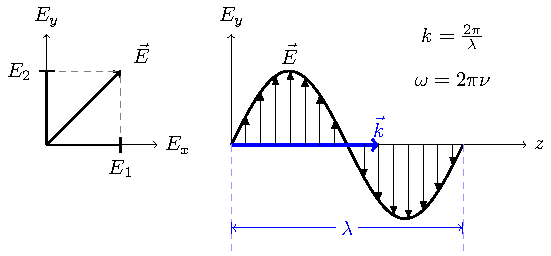
\includegraphics[width=0.7\textwidth]{img/e}
	\end{center}
\end{frame}
%%%%%%%%%%%%%%%%%%%%%%%%%%%%%%%%
	% \begin{columns}
	% 	\begin{column}{0.5\textwidth}

	% 	\end{column}
	% 	\begin{column}{0.5\textwidth}

	% 	\end{column}
	% \end{columns}
%%%%%%%%%%%%%%%%%%%%%%%%%%%%%%%%%%%%%%%%%%%%%%%%%%%%%%%%%%

\begin{frame}
	\begin{columns}
		\begin{column}{0.7\textwidth}
			\begin{enumerate}
			\item Если $\delta=0, \pi$, то
			% $\frac{E_x^2}{E_1^2}\pm\frac{2E_xE_y}{E_1E_2}+\frac{E_y^2}{E_2^2}=0$\\
			\begin{equation*}				
				\frac{E_x}{E_1}\pm\frac{E_y}{E_2}=0
			\end{equation*}
			% \\
			-- \textbf{линейная} поляризация.
			\vspace{1em}
			\item Если $\delta=\frac{\pi}{2}$, то\\
			\begin{equation*}				
				\frac{E_x^2}{E_1^2}+\frac{E_y^2}{E_2^2}=1				
			\end{equation*}			
			-- \textbf{эллиптическая} поляризация, которая при $E_1=E_2 \equiv E'$ переходит в \textbf{круговую}:
			\begin{equation*}				
				E_x^2+E_y^2=E'^2
			\end{equation*}			
			\end{enumerate}	
			C понятием поляризации тесно связано явление \textbf{двойного лучепреломления}.
		\end{column}
		\begin{column}{0.3\textwidth}
			\begin{tikzpicture}
				\draw[black, thick] (-1,-1) -- (1,1);% node[above, xshift=1em] {$\vec{E}$};
				\draw[black, thick] (1,-1) -- (-1,1);% node[above, xshift=1em] {$\vec{E}$};
				\draw[dashed, black!50] (1,0) -- (1,1);
				\draw[dashed, black!50] (0,1) -- (1,1);

				\draw[dashed, black!50] (-1,1) -- (0,1);
				\draw[dashed, black!50] (-1,1) -- (-1,0);

				\draw[black,->, thin] (-1.5,0) -- (1.5,0) node [right] {$E_x$};
				\draw[black,->, thin] (0,-1.5) -- (0,1.5) node [above] {$E_y$};

				% \draw[black,-,thick] (0,0) -- ++(1,0);
				% \draw[black,-,thick] (0,0) -- ++(0,1);

				\draw[black,thick] (1,-.1) node[below] {${E}_1$} -- ++(0,0.2);
				\draw[black,thick] (-1,-.1) node[below] {$-{E}_1$} -- ++(0,0.2);
				\draw[black, thick] (-.1,1) node[left,yshift=0.6em] {${E}_2$} -- ++(0.2,0);
				\draw[black,-latex, thick] (0,0) -- (1,{sqrt(1)}) node[above, xshift=0em] {$\vec{E}$};
				\draw[black,-latex, thick] (0,0) -- (135:1);				
				\draw[black,-latex, thick] (0,0) -- (135:1);				
			\end{tikzpicture}
			\begin{tikzpicture}

				\draw[black,-latex, thick] (0,0) -- (1,0.71) node[above, xshift=0em] {$\vec{E}$};
				\draw[black,-latex, thick] (0,0) -- (130:1);
				% \draw[black, thick] (1,-1) -- (-1,1);% node[above, xshift=1em] {$\vec{E}$};
				\draw[thick] (0,0) circle (1);
				\draw[thick] (0,0) ellipse (1.4 and 1);
				% \draw[dashed, black!50] (1,0) -- (1,1);
				% \draw[dashed, black!50] (0,1) -- (1,1);

				% \draw[dashed, black!50] (-1,1) -- (0,1);
				% \draw[dashed, black!50] (-1,1) -- (-1,0);

				\draw[black,->, thin] (-1.5,0) -- (1.5,0) node [right] {$E_x$};
				\draw[black,->, thin] (0,-1.5) -- (0,1.5);% node [above] {$E_y$};

				% \draw[black,-,thick] (0,0) -- ++(1,0);
				% \draw[black,-,thick] (0,0) -- ++(0,1);

				% \draw[black,thick] (1,-.1) node[below] {${E}_1$} -- ++(0,0.2);
				% \draw[black,thick] (-1,-.1) node[below] {$-{E}_1$} -- ++(0,0.2);
				% \draw[black, thick] (-.1,1) node[left,yshift=0.6em] {${E}_2$} -- ++(0.2,0);
			\end{tikzpicture}			
		\end{column}
	\end{columns}
	
\end{frame}

%%%%%%%%%%%%%%%%%%%%%%%%%%%%%%%%%%%%%%%%%%%%%%%%%%%%%%%%%%%%%
\begin{frame}[t]
	\subsection{Понятие двулучепреломления}
	\frametitle{Понятие двулучепреломления}
	% ЧТО ТАКОЕ ДВУЛУЧЕПРЕЛОМЛЕНИЕ
	% ИЗОТРОПНОЕ СТЕКЛО ДВУЛУЧЕПРЕЛОМЛЕНИЕ% ИЗ-ЗА МАГНИТНОГО ПОЛЯ
	% КАРТИНКА ИЗ СИВУХИНА
	% ЦИРКУЛЛЯРНОЕ ДВУЛУЧЕПРЕЛОМЛЕНИЕ
	\begin{enumerate}
		\item \textbf{Двойное лучепреломление} — раздвоение светового луча при прохождении через анизотропную среду, обусловленное зависимостью показателя преломления от поляризации волны и ориентации волнового вектора. 
			\begin{figure}[tb]
				\centering
				% 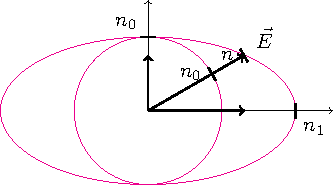
\includegraphics[width=\textwidth]{img/dvp2}
				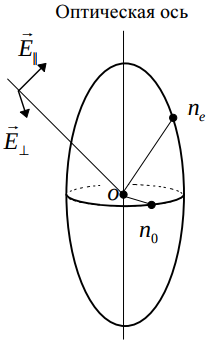
\includegraphics[width=0.2\textwidth]{img/ell}
			\end{figure}		
		\item Вращение плоскости поляризации есть проявление \textbf{особого двулучепреломления -- кругового}. В этом случае обыкновенная и необыкновенная волны будут поляризованы циркулярно.
	\end{enumerate}


\end{frame}
%%%%%%%%%%%%%%%%%%%%%%%%%%%%%%%%%%%%%%%%%%%%%%%%%%%%%%%%%%%%%

\begin{frame}[t]
	\begin{enumerate}
		\item \textbf{Круговое двулучепреломление}. Предположим, что угол поворота поляризации зависит от $z$ как 
$\Theta=-\alpha z$. Тогда можно показать, что волну с повернувшейся поляризацией можно представить как суперпозицию поляризованных по левому ($L$) и правому ($R$) кругу волн, и для них
\begin{gather*}
	v_L=\frac{\omega}{k-\alpha},
	\quad
	v_R=\frac{\omega}{k+\alpha},
	\quad
	n_L=\frac{c}{v_L},
	\quad
	n_R=\frac{c}{v_L}
\end{gather*}
откуда выражается
\begin{equation*}
	\alpha=\frac{\omega}{2c}(n_L-n_R)
\end{equation*}
\item В магнитном поле у вещества существуют \textbf{собственные частоты} ($\omega_0\pm\Omega$),
и по Френелю это и есть причина поворота поляризации: сложение двух таких циркулярно поляризованных волн даст волну с повернутой линейной поляризацией
\begin{equation*}
	\Theta=\frac{\pi L}{\lambda}(n_--n_+)
\end{equation*}
		\item \textbf{Эффект Фарадея} заключается в возникновении кругового двулучепреломления в изначально изотропных средах при \\помещении их в магнитное поле. 
	\end{enumerate}
	% указать что омега ларморовская
	% \begin{columns}
	% 	\begin{column}{0.5\textwidth}	
			
	% 		\begin{gather*}
	% 			n_{1,2}=\frac{c}{V_{1,2}}
	% 			% V_{1,2}=\frac{\lambda}{t_{1,2}}\\
	% 			% \alpha_{1,2}=\omega (t_{1,2}-t)
	% 		\end{gather*}
			
	% 	\end{column}
	% 	\begin{column}{0.5\textwidth}
	% 		\begin{figure}[tb]
	% 			\centering
	% 			% 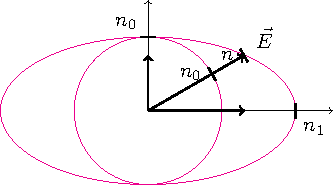
\includegraphics[width=\textwidth]{img/dvp2}
	% 			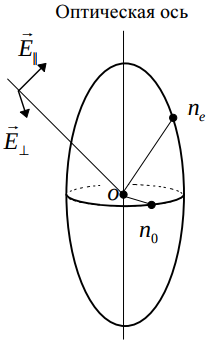
\includegraphics[width=0.4\textwidth]{img/ell}
	% 		\end{figure}
	% 	\end{column}
	% \end{columns}
\end{frame}

%%%%%%%%%%%%%%%%%%%%%%%%%%%%%%%%%%%%%%%%%%%%%%%%%%%%%%%%%%%%%
\begin{frame}[t]
	\subsection{Вращатели Фарадея}
	%
	\frametitle{Вращатель и изолятор Фарадея}
	% \framesubtitle{Вращение плоскости поляризации}
	\textbf{Вращатель Фарадея} - устройство, способное вращать плоскость поляризации в магнитном поле. \textbf{Изолятор Фарадея} - устройство, поворачивающее плоскость поляризации на $\frac{\pi}{4}$. 
	% \vspace{1em}
	\begin{center}
		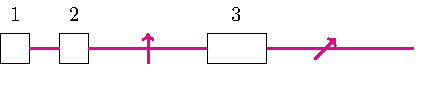
\includegraphics[width=0.8\textwidth]{img/rot}\\
		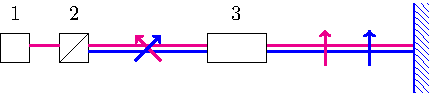
\includegraphics[width=0.8\textwidth]{img/zerc}
	\end{center}
	\begin{columns}
		\hspace{2.5cm}
		\begin{column}{0.3\textwidth}
			
			\textbf{1} -- источник
			
			\textbf{2} -- поляризатор
			
		\end{column}
		\hspace{1.6cm}
		\begin{column}{0.7\textwidth}
			
			\textbf{3} -- вращатель\\
			или изолятор Фарадея
		\end{column}
	\end{columns}
	% НАРИСОВАТЬ ПОЛЯРИЗАТОР НА РИСУНКЕ УГОЛ ПОВОРОТА ПЛ ПОЛЯРИЗАЦИИ
	% МАГНИТ С МАГНИТОАКТИВНЫМ МАТЕРИАЛОМ (МАГНИТНАЯ СИСТЕМА)
	% \textbf{1} -- источник
	
	% \textbf{2} -- поляризатор
	
	% \textbf{3} -- вращатель/фильтр Фарадея
	
\end{frame}
%%%%%%%%%%%%%%%%%%%%%%%%%%%%%%%%%%%%%%%%%%%%%%%%%%%%%%%%%%%%%
\begin{frame}
	\frametitle{Материальная константа: постоянная Верде}
	$V$ -- \textbf{постоянная Верде} -- физическая величина, характеризующая угол, на который повернется плоскость поляризации при данных длине образца и магнитном поле:
	% КАРТИНКА: нарисовать плоскость поляризации и угол, на к-й она поворачивается
	\begin{equation}
		\Theta=\varphi_2-\varphi_1=V \int B(z)dz
	\end{equation}
	где $\Theta$ -- угол, на который поворачивается плоскость поляризации.
	\begin{center}
		% 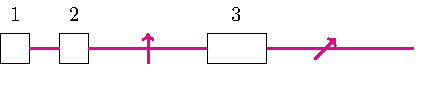
\includegraphics[width=0.8\textwidth]{img/rot}\\
		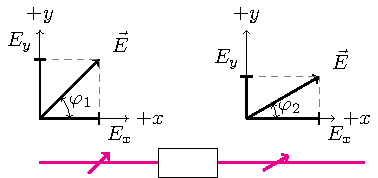
\includegraphics[width=0.8\textwidth]{img/rotpol}
	\end{center}
	% МАГНИТНАЯ СИСТЕМА
\end{frame}
%%%%%%%%%%%%%%%%%%%%%%%%%%%%%%%%%%%%%%%%%%%%%%%%%%%%%%%%%%%%%
\section{Экспериментальная часть}
\begin{frame}
	\subsection{Схема установки}
	\frametitle{Схема установки}
	\begin{figure}[tb]
		\centering
		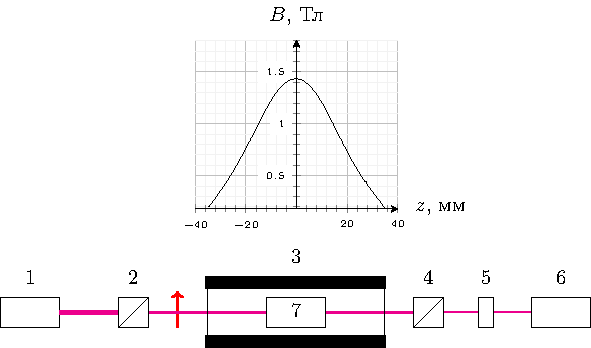
\includegraphics[width=0.8\textwidth]{img/chem}
	\end{figure}
	\begin{columns}
		\hspace{2.5cm}
		\begin{column}{0.3\textwidth}
			\textbf{1} -- диодный лазер\\ 
			$\quad\lambda_1=531$ нм,\\
			$\quad\lambda_2=658$ нм,\\
			$\quad\lambda_3=1064$ нм\\
			\textbf{2} -- поляризатор
		\end{column}
		\hspace{1.6cm}
		\begin{column}{0.7\textwidth}
			\textbf{3} -- магнит\\
			\textbf{4} -- призма Глана\\
			\textbf{5} -- фильтр\\
			\textbf{6} -- камера\\
			\textbf{7} -- образец
		\end{column}
	\end{columns}
	% ПОКАЗАТЬ ПОЛЯРИЗАЦИЮ ПОСЛЕ ВРАЩАТЕЛЯ
\end{frame}
%%%%%%%%%%%%%%%%%%%%%%%%%%%%%%%%%%%%%%%%%%%%%%%%%%%%%%%%%%%
\begin{frame}
	\subsection{Аппроксимация распределения магнитного поля}
	\frametitle{Аппроксимация распределения магнитного поля}
	Мы аппроксимировали полученное распределение $B(z)$ с помощью кривой Гаусса:
	\begin{center}
	\hspace{4em}
	\begin{tikzpicture}[scale=1.3]
\begin{axis}[
    xlabel={$z$, мм},
    ylabel={$B$, Тл},
    scale=0.5,
    grid=both,
    grid style={line width=.1pt, draw=gray!10},
    major grid style={line width=.2pt,draw=gray!50},
    minor y tick num=4,
    minor x tick num=4,   
    xtick distance=20,
    ytick distance=.5,
    domain=-40:40,
    ymax = 1.8,
    xmin = -40,
    xmax = 40,
    ticklabel style={font=\tiny,fill=white},    
    axis lines=middle,     
  every axis x label/.style={
      at={(ticklabel* cs:1.05)},
      anchor=west,
  },
  every axis y label/.style={
      at={(ticklabel* cs:1.05)},
      anchor=south,
  },    
  /pgf/number format/.cd,
  use comma,
  restrict y to domain=0:1.5,
  set decimal separator={.},
    1000 sep={}, 
    ]  
  \addplot[mark=*,mark size=0.2] table [x=l, y=10t, col sep=tab] {data/b_x.csv}; 
  \addplot[smooth, red] {1.428*exp(-((x+0.2581)/25.06)^2)};
  \end{axis} 
	\end{tikzpicture}
	\end{center}
\begin{equation*} 
B=B_0%\frac{1}{\sigma\sqrt{2\pi}} 
\exp 
\left[ 
- (x-\mu)^2
\cdot
B^2_0\pi 
\right], 
\end{equation*}
где $B_0=1.433$ Тл, а $\mu=-0.2581$ мм.
%$\mu=-0.2581\pm0.03$, $\sigma=17.72\pm0.05$
% ЗАМЕНИТЬ КОНСТАНТЫ ВВЕСТИ В0 НАПИСАТЬ РАЗМЕРНОСТИ
% $	a1 = 1.428;%  (1.425, 1.43)
% b1 = -0.2581;%  (-0.2927, -0.2235)
% c1 = 25.06;%  (25, 25.11)
% FF=@(x)  a1.*exp(-((x-b1)./c1).^2);$
\end{frame}
%%%%%%%%%%%%%%%%%%%%%%%%%%%%%%%%%%%%%%%%%%%%%%%%%%%%%%%%%%
\begin{frame}[t]
	\subsection{Анализ результатов}
	\frametitle{Результаты эксперимента}
	% \begin{columns}
	% \begin{column}{0.4\textwidth}
	% 	\tikz{\draw[fill=magenta] (0,0) rectangle (0.5em,0.5em);} — \small{TWLTb-231/1 (l=25.8мм)}\\
	% 	\tikz{\draw[fill=blue] (0,0) rectangle (0.5em,0.5em);} — \small{TWLDyB-235/4 (15,2мм)}\\
	% 	\tikz{\draw[fill=black] (0,0) rectangle (0.5em,0.5em);} — \small{TWLPB-229/1 (22,5мм)}\\
	% 	\tikz{\draw[fill=green] (0,0) rectangle (0.5em,0.5em);} — \small{TWLEuB-230/6 (20,2мм)}\\
	% 	\tikz{\draw[fill=magenta!40!blue] (0,0) rectangle (0.5em,0.5em);} — \small{TZNDy-236/4 (24,7мм)}\\
	% 	Лучший образец -- TZNDy-236/4\\
	% 	Худший -- TWLTb-231/1
	% \end{column}
	% \begin{column}{0.6\textwidth}
	\begin{figure}[tb]
		\centering
		% \hspace{5em}%!TEX root = presa.tex
  \begin{tikzpicture}[scale=1.1]
  \begin{axis}[
    xlabel={$\lambda$, нм},
    ylabel={$V, \frac{\text{рад}}{\text{Тл}\cdot\text{м}}$},
    domain=400:2000,
    grid=both,
    grid style={line width=.1pt, draw=gray!10},
    major grid style={line width=.2pt,draw=gray!50},
    minor y tick num=4,
    minor x tick num=4,
    xtick distance=200,
    ytick distance=5,
    ymin = 4,
    % enlargelimits={abs=0.5},
    axis line style={latex-latex},
    ticklabel style={font=\small,fill=white},    
    axis lines=middle,     
    % legend pos = north west,
    legend entries={{TWLTb-231/1},
                    {TWLDyB-235/4},
                    {TWLPB-229/1},
                    {TWLEuB-230/6},
                    {TZNDy-236/4}},
    % legend pos=outer north east    
    legend pos= north east,  
every axis x label/.style={
    at={(ticklabel* cs:1.05)},
    anchor=west,
},
every axis y label/.style={
    at={(ticklabel* cs:1.05)},
    anchor=south,
},    
   /pgf/number format/.cd,
        use comma,
        1000 sep={}]
    % legend style={
    % at={(0,0)},
    % anchor=north east,at={(axis description cs:0,-0.1)}},
    % ]

  \addlegendimage{mark=square*,color=magenta}
  \addlegendimage{mark=*,color=blue,dashed}
  \addlegendimage{mark=otimes,color=black}
  \addlegendimage{mark=triangle*,color=red}
  \addlegendimage{mark=diamond*,color=magenta!40!blue}

  \xdef\A{1.163e+04}
  \xdef\B{0.6811}
  \xdef\C{0.09754}

  \addplot[magenta]{1/x*(\A+\B/(x^2-\C^2))};    
    \addplot[color=magenta, draw=none,mark=square*] coordinates {
    (531,22.8)
    (658,13.24)
    (1064,9.36)
  };
 \xdef\A{1.35e+04} 
\xdef\B{0.5606} 
\xdef\C{0.9575} 
  \addplot[blue,dashed]{1/x*(\A+\B/(x^2-\C^2))};    
    \addplot[color=blue, draw=none,mark=*] coordinates {
    (531,31.74)
    (658,15.25)
    (1064,5.48)
  };  
\xdef\A{1.219e+04} 
\xdef\B{0.1984} 
\xdef\C{0.9706} 
  \addplot[black]{1/x*(\A+\B/(x^2-\C^2))};    
    \addplot[color=black, draw=none,mark=otimes] coordinates {
    (531,24.3)
    (658,14.05)
    (1064,10.36)
  };  
\xdef\A{1.469e+04} 
\xdef\B{0.4854} 
\xdef\C{0.8003} 
  \addplot[red]{1/x*(\A+\B/(x^2-\C^2))};    
    \addplot[color=red, draw=none,mark=triangle*] coordinates {
    (531,29.58)
    (658,17.12)
    (1064,12.79)
  };   
\xdef\A{1.679e+04} 
\xdef\B{0.4218} 
\xdef\C{0.9157}
  \addplot[magenta!40!blue]{1/x*(\A+\B/(x^2-\C^2))};    
    \addplot[color=magenta!40!blue, draw=none,mark=diamond*] coordinates {
    (531,30.77)
    (658,19.68)
    (1064,11.69)
  };        

  \end{axis}
  \end{tikzpicture}    
		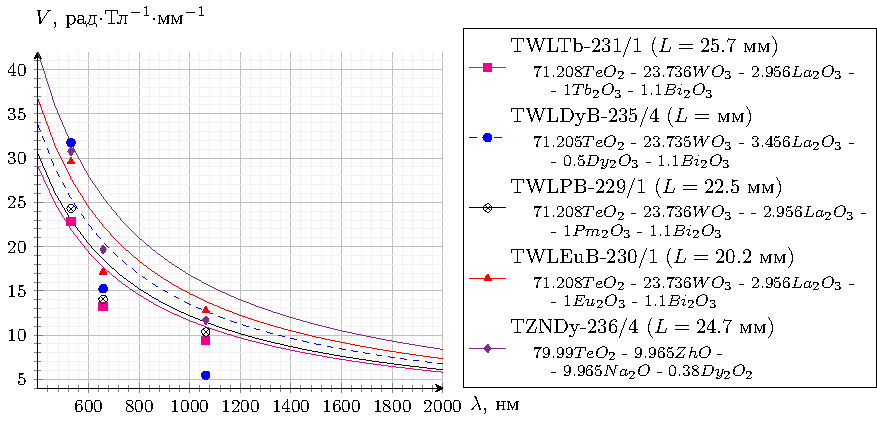
\includegraphics[width=1\textwidth]{images/graph_verde_from_lambda}
	\end{figure}
	% ПОДПИСАТЬ ДЛИНЫ И СОСТАВЫ ОБРАЗЦОВ
	% ДОБАВИТЬ СЮДА ОЦЕНКУ И УБРАТЬ ОТТУДА ТЕКСТ
	% \end{column}
	% \end{columns}
	% \begin{itemize}
		% \item 
		\textbf{Оценка} образца TZNDy-236/4: Для поворота на $\Theta=\frac{\pi}{4}$ при $B=3.5$ Тл и длине волны $\lambda=1800$ нм нужен образец длиной 2 см.
	% \end{itemize}
\end{frame}
%%%%%%%%%%%%%%%%%%%%%%%%%%%%%%%%%%%%%%%%%%%%%%%%%%%%%%%%%%%%%
% \begin{frame}
% 	\subsection{Оценка}
% 	\frametitle{Оценка}
% 	(ЭТО ОТТУДА ЗДЕСЬ)
% 		$\quad \Theta=VBL$\\
% 		$\quad L=\frac{\Theta}{VB}$\\
% 		$\quad B=3.5$ Тл\\
% 		$\quad \Theta=\frac{\pi}{4}$\\
% 		$\quad \lambda=1.8$ мкм\\
% 		$\quad V=9.3$ \\
% 		$\quad L=2$ см\\
% 	Для оценки был выбран образец с наибольшей материальной константой, так как он на наибольший угол поворачивает плоскость поляризации.\\

% 	Длина образца с составом TZNDy-236/4, при которой плоскость поляризации повернулась бы на $\frac{\pi}{4}$ -- 2см для волны 1,8мкм.\\	

% 	При такой длине образца неоднородность магнитного поля сказываться не будет, следовательно, как изолятор Фарадея его эффективно применять при таком магнитном поле.
	
% \end{frame}
%%%%%%%%%%%%%%%%%%%%%%%%%%%%%%%%%%%%%%%%%%%%%%%%%%%%%%%%%%%%%
\section{Выводы}
\begin{frame}
	\frametitle{Выводы}
	В этой работе 
		\begin{enumerate}
		\item исследовали магнитооптические свойства теллуритных стекол (определили постоянную Верде)
		\item оценили длину образца, при которой теллуритное стекло вместе с магнитной системой стали бы изолятором Фарадея
	\end{enumerate}
\end{frame}

\begin{frame}[plain]
	\vspace{4cm}
	\begin{center}
		\Huge
		Спасибо за внимание!
	\end{center}
	\vspace{2.5cm}
	\begin{center}
		\color{black!30!white}
		Презентация подготовлена в издательской \\
		системе LaTeX с использованием пакетов \\
		PGF/TikZ и Beamer
	\end{center}
\end{frame}

% \begin{frame}[t]
	
% \end{frame}
\begin{frame}
% \subsection{Понятие поляризации}
	\frametitle{Сложение взаимно перпендикулярных гармонических колебаний}
Рассмотрим уравнение волны: 
\begin{gather*} 
\begin{cases} 
E_x = E_1\cos\left(-kz+\omega t+\varphi_1\right) \\ 
E_y = E_2\cos\left(-kz+\omega t+\varphi_2\right) \\ 
E_z = 0 
\end{cases} 
\end{gather*} 
Исключим из них время. Для этого 
\begin{enumerate} 
\item % 
$\frac{E_x}{E_1}=\cos(-{k}{z}+\omega t)\cos\varphi_1-\sin(-kz+\omega t)\sin\varphi_1$\\ %(*) 
$\frac{E_y}{E_2}=\cos(-kz+\omega t)\cos\varphi_2-\sin(-kz+\omega t)\sin\varphi_2$ %(**) 
\item %Умножив выражение (*) на $\cos\varphi_2$ и (**) на $\cos\varphi_1$ после вычитания из первого равенства второго, получим: 
$\frac{E_x}{E_1}\cos\varphi_2-\frac{E_y}{E_2}\cos\varphi_1=\sin(-kz+\omega t)\sin(\varphi_2-\varphi_1)$ 
\item %Теперь умножим выражение (*) на $\sin\varphi_2$ , а (**) на $\sin\varphi_1$ и также вычтем з первого равенства второе 
$\frac{E_x}{E_1}\sin\varphi_2-\frac{E_y}{E_2}\sin\varphi_1=\sin(-kz+\omega t)\sin(\varphi_2-\varphi_1)$ 
\item %Возведя в квадрат и сложив почленно последние два уравнения, получим уравнение траектории 
$\frac{E_x^2}{E_1^2}-\frac{2E_xE_y}{E_1E_2}\cos(\varphi_2-\varphi_1)+\frac{E_y^2}{E_2^2}=\sin(\varphi_2-\varphi_1)$, 
$\varphi_2-\varphi_1=\delta$ 
\item $\frac{E_x^2}{E_1^2}-\frac{2E_xE_y}{E_1E_2}\cos\delta+\frac{E_y^2}{E_2^2}=\sin^2\delta$ 
\end{enumerate} 
% А это уравнение эллипса.

% Следовательно, поляризация в общем случае эллиптическая. ЧТО ТАКОЕ Е1 И Е2 ИСПРАВИТЬ НА РИСУНКЕ ИСПРАВИТЬ РИСУНОК:
% УБРАТЬ ПЛЮСЫ
% ВОЛНОВОЙ ВЕКТОР
\end{frame}

%%%%%%%%%%%%%%%%%%%%%%%%%%%%%%%%%%%%%%%%%%%%%%%%%%%%%%%%%%%%%
\end{document}

1. влияние состава стекол
влияет примесь .
Размер - апертура (какой размер, сколько можно) (до 10 и слава богу)
